% !TEX root = sum1.tex
\section{Seat Planning Problem with Social Distancing}\label{problem_description}
We formally describe the problem of considering social distancing measures in the seat planning process. We first introduce some concepts, then present an optimization model for the problem with deterministic requests.

\subsection{Concepts}
Consider a seat layout comprising $N$ rows, with each row $j$ containing $L_j^0$ seats, for  $j \in \mathcal{N} \coloneqq \{1,2, \ldots, N\}$. The venue will hold an event with multiple seat requests, where each request includes a group of multiple people.
There are $M$ distinct group types, where each group type $i$, $i \in \mathcal{M} \coloneqq \{1, 2, \ldots, M\}$, consists of $i$ individuals requiring $i$ consecutive seats in one row. The request of each group type is represented by a demand vector $\mathbf{d} = (d_1, d_2, \ldots, d_M)^{\intercal}$, where $d_i$ is the number of groups of type $i$.

To adhere to social distancing requirements, individuals from the same group must sit together in one specific row while maintaining a distance, measured by the number of empty seats, from adjacent groups in the same row.
Let $\delta$ denote the social distance, which could entail leaving one or more empty seats. Specifically, each group must ensure the empty seat(s) with the adjacent group(s). To model the social distancing requirements into the seat planning process, we define the size of group type $i$ as $n_i = i + \delta$, where $i \in \mathcal{M}$. Correspondingly, the size of each row is defined as $L_j = L_j^{0} + \delta$. It is a clear one-to-one mapping between the original physical seat plan and the model of seat plan. By incorporating the additional seat(s) and designating certain seat(s) for social distancing, we can integrate social distancing measures into the seat plan problem.

Since each group occupies only one row, we assume that the physical distance between different rows is sufficient. If the social distancing requirement is more stringent, an empty row can be implemented, as practiced by some theaters \citep{Berlin_theater}.

We introduce the term \textit{pattern} to describe the seat planning arrangement for a single row. A specific pattern can be represented by a vector $\bm{h} = (h_1, \ldots, h_M)$, where $h_i$ denotes the number of groups of type $i$ in the row for $i = 1,\ldots, M$. A feasible pattern, $\bm{h}$, must satisfy the condition $\sum_{i=1}^{M} h_i n_i \leq L$ and belong to the set of non-negative integer values, denoted as $\bm{h} \in \mathbb{N}^{M}$. A seat plan with $N$ rows can be represented as $\bm{H} = [\bm{h}_{1}^{\intercal}, \ldots, \bm{h}_{N}^{\intercal}]$, where each element, $H_{ij}$, denotes the number of groups of type $i$ planned in row $j$. The supply of the seat plan is represented by $\bm{X} = (X_{1}, \ldots, X_{M})^{\intercal}$, where $X_i= \sum_{j=1}^{N} H_{ij}$ indicates the supply for group type $i$. In other words, $\bm{X}$ captures the number of groups of each type that can be accommodated in the seat layout by aggregating the supplies across all rows.

Let $|\bm{h}|$ denote the maximum number of individuals that can be assigned according to pattern $\bm{h}$, i.e., $|\bm{h}| = \sum_{i =1}^{M} i h_i$. The size of $\bm{h}$, $|\bm{h}|$, serves as a measure of the maximum seat occupancy achievable under social distancing constraints. By analyzing $|\bm{h}|$ across different patterns, we can evaluate the effectiveness of various seat plan configurations in accommodating the desired number of individuals while complying with social distancing requirements.

The above description can be illustrated by the example in Fig.~\ref{fex1}.

\begin{example}
Consider a single row of $L^0=10$ seats and the social distancing requirement of $\delta = 1$ empty seat between groups. There are four groups, groups 2 and 4 in group type 1, group 1 in type 2, and group 3 in type 3.
\end{example}

\begin{figure}[ht]
    \centering
        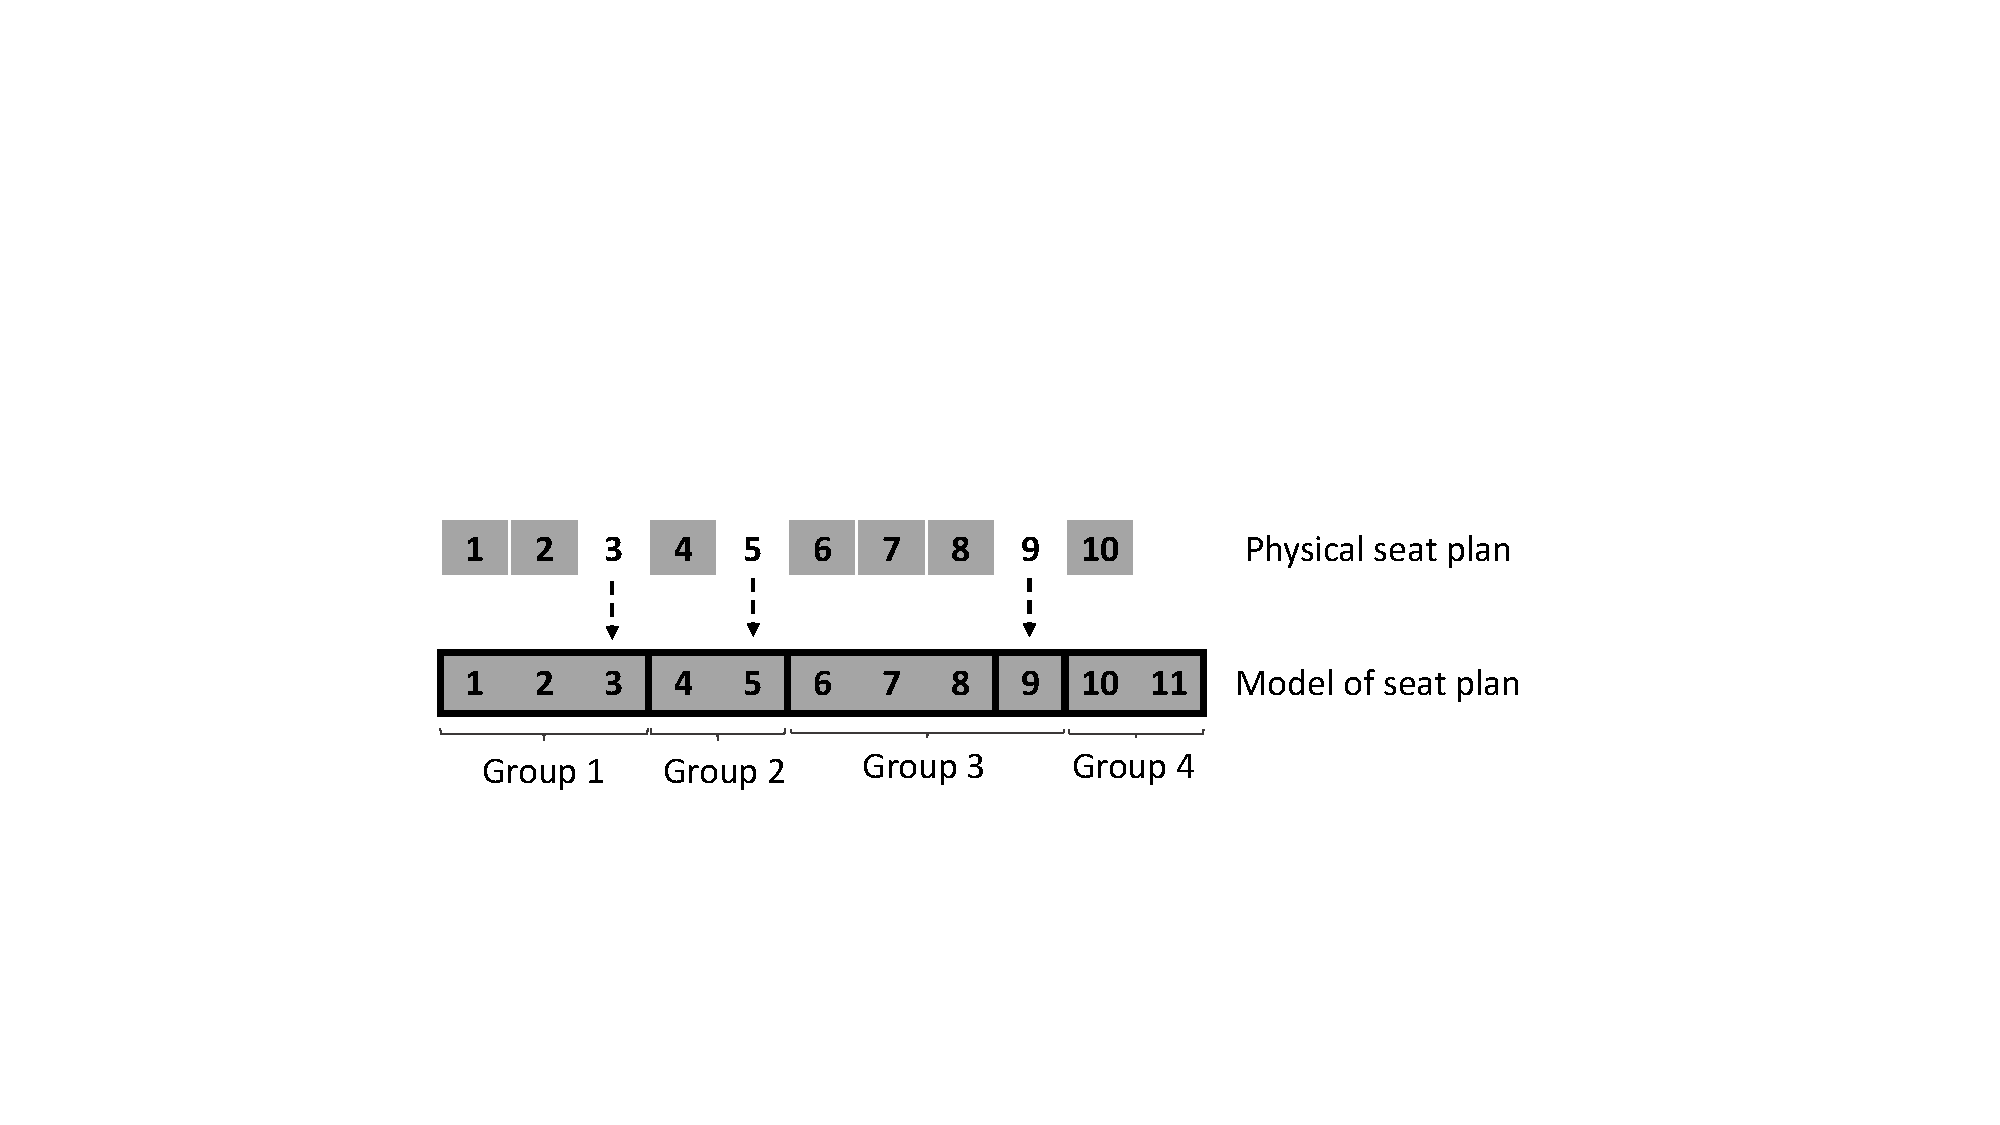
\includegraphics[width=0.55\textwidth]{./Figures/model_plan.pdf}
    \caption{Illustration of Groups with Social Distancing}\label{fex1}
\end{figure}

In the model, the size of the row is $L = L^{0} + \delta =11$. The seat plan for the row can be represented by $\bm{h} = (2,1,1,0)$ with $|\bm{h}| = 7$.

SPDRP can be formulated by an integer programming, where we define $x_{ij}$ to be the number of groups of type $i$ planned in row $j$.

\begin{align}
    \max \quad & \sum_{i=1}^{M}  \sum_{j= 1}^{N} (n_i- \delta) x_{ij} \label{e0} \\
    \text {s.t.} \quad & \sum_{j= 1}^{N} x_{ij} \leq d_{i}, \quad i \in \mathcal{M}, \label{deter_upper}\\ 
    & \sum_{i=1}^{M} n_{i} x_{ij} \leq L_j, j \in \mathcal{N}, \label{capa_con} \\
    & x_{ij} \in \mathbb{N}, \quad i \in \mathcal{M}, j \in \mathcal{N}. \notag 
\end{align}

The objective is to maximize the number of individuals accommodated. Constraint \eqref{deter_upper} ensures the number of accommodated groups does not exceed the number of requests. Constraint \eqref{capa_con} stipulates that the number of seats allocated in each row does not exceed the size of the row.

By examining the monotonic ratio between the original group sizes and the adjusted group sizes, we can establish the upper bound of supply corresponding to the optimal solution of the LP relaxation of SPDRP. This is illustrated in Proposition \ref{sol_relax_deter} and will be utilized in the bid-price control policy discussed in Appendix \ref{policies}.

\begin{prop}\label{sol_relax_deter}
For the LP relaxation of \textup{SPDRP}, there exists an index $\tilde{i}$ such that the optimal solutions satisfy the following conditions: $x_{ij}^{*} = 0$ for all $j$, $i = 1,\ldots, \tilde{i}-1$; $\sum_{j} x_{ij}^{*} = d_{i}$ for $i = \tilde{i}+1,\ldots, M$; $\sum_{j} x_{ij}^{*} = \frac{L - \sum_{i = \tilde{i}+1}^{M} {d_i n_i}}{n_{\tilde{i}}}$ for $i = \tilde{i}$.
\end{prop}

In other words, the supply corresponding to the optimal solutions for group types $i$ (where $i > \tilde{i}$) exactly matches the demand of group type $i$. For group types $i$ (where $i < \tilde{i}$), the supply is zero. The supply for group type $\tilde{i}$ is determined by the remaining available seats.

\subsection{Seat Planning with Full or Largest Patterns}\label{seat_planning_full_largest}
While the IP (\ref{e0}) is not difficult to solve for any practical problem, the optimal solution reveals some interesting observations regarding the structure  of the optimal seat plan. In particular, when some constraints \eqref{deter_upper} are not tight, most constraints (\ref{capa_con}) tend to be tight. In words, if some requests are rejected, the seats in each row tend to be fully used. Note that each constraint in \eqref{capa_con} corresponds to a pattern of a row.
This leads to the following definition.

\begin{definition}
Consider a pattern $\bm{h} = (h_1, \ldots, h_M)$ for a row of size $L$. We say $\bm{h}$ to be a full pattern if $\sum_{i=1}^{M} n_i h_i = L$, and $\bm{h}$ to be a largest pattern if its size $|\bm{h}| \geq |\bm{h}^{\prime}|$, for any other feasible pattern $\bm{h}^{\prime}$.
\end{definition}

The above concepts characterize two types of tightness of a pattern. In a full pattern, the corresponding constraint is mathematically tight. In a  maximum pattern, the mathematical tightness is not enforced on the constraint; instead, it is reflected with respect to the objective function in that any other pattern cannot lead to a higher objective function   value. Both the full pattern and the maximum pattern imply the efficient use of the seats and shall be used in an optimal seat plan.

\begin{prop}\label{lem_pattern}
The size of a largest pattern, denoted by $\phi(M, L^{0}, \delta)$ as a function of $M$, $L^{0}$ and $\delta$, is given by $$\phi(M, L^{0}, \delta) = q M + \max\{r-\delta, 0\},$$ where $q$ is the quotient of $(L^{0} + \delta)$ divided by $(M+\delta)$ and $r$ is the remainder. In addition, $\phi(M,L)$ is non-decreasing with $M$, $L$ and $\delta$, respectively. 
\end{prop}

The size, $qM + \max\{r-\delta, 0\}$, corresponds directly to a largest pattern that includes $q$ group type $M$ and $r$ seats for one group type $(r-\delta)$ when $r>\delta$. However, the form of the largest pattern is not unique; there are other largest patterns that share the same size. 
Specifically, when $r = 0$, the largest pattern is unique and full, indicating that only one pattern can accommodate the maximum number of individuals; when $r > \delta$, the largest pattern is full, as it uses all available seats.

A concept closely related to the largest pattern is the \textit{maximum achievable occupancy rate}.
For a single row, the rate is $\frac{\phi(M, L^{0}, \delta)}{L^{0}}$, and this can be extended to $N$ rows. The maximum achievable occupancy rate is attained when each row of a given layout is a largest pattern. This rate is defined as:

$$\frac{\sum_{j \in \mathcal{N}}\phi(M, L_{j}^{0}; \delta)}{\sum_{j \in \mathcal{N}} L_{j}^{0}},$$
where $\phi(M, L^{0}, \delta)$ represents the size of the largest pattern under $M$, $L$ and $\delta$.

\begin{corollary}\label{maximum_phi}
The maximum achievable occupancy rate is non-decreasing in $M$ and $\delta$, but not monotone in $L_{j}^{0}, \forall j \in \mathcal{N}$.
\end{corollary}


According to Proposition \ref{lem_pattern}, $\phi(M, L^{0}, \delta)$ is non-decrease in $M$. When $M$ increases, the maximum achievable occupancy rate does not decrease. Similarly, the maximum achievable occupancy rate does not decrease when $\delta$ increases. Although $\phi(M, L^{0}, \delta)$ is non-decreasing in $L$, for a single row, when $L$ increases while $M$ remains unchanged, the maximum achievable occupancy rate may either increase or decrease. Consequently, the trend of the maximum achievable occupancy rate for a layout is not straightforward. Further discussion on the maximum achievable occupancy rate will be provided in Section \ref{impact_sd}.

\begin{example}
Consider the given values: $\delta = 1$, $L = 21$, and $M = 4$. The size of the largest pattern can be calculated as $qM + \max\{r-\delta, 0\} = 4 \times 4 + 0 = 16$. The largest patterns are as follows: $(1, 0, 1, 3)$, $(0, 1, 2, 2)$, $(0, 0, 0, 4)$, $(0, 0, 4, 1)$, and $(0, 2, 0, 3)$. Among these, $(0, 0, 0, 4)$ is the form referenced in Proposition \ref{lem_pattern}.

The following figure shows that the largest pattern may not be full and the full pattern may not be largest.
\begin{figure}[ht]
    \centering
        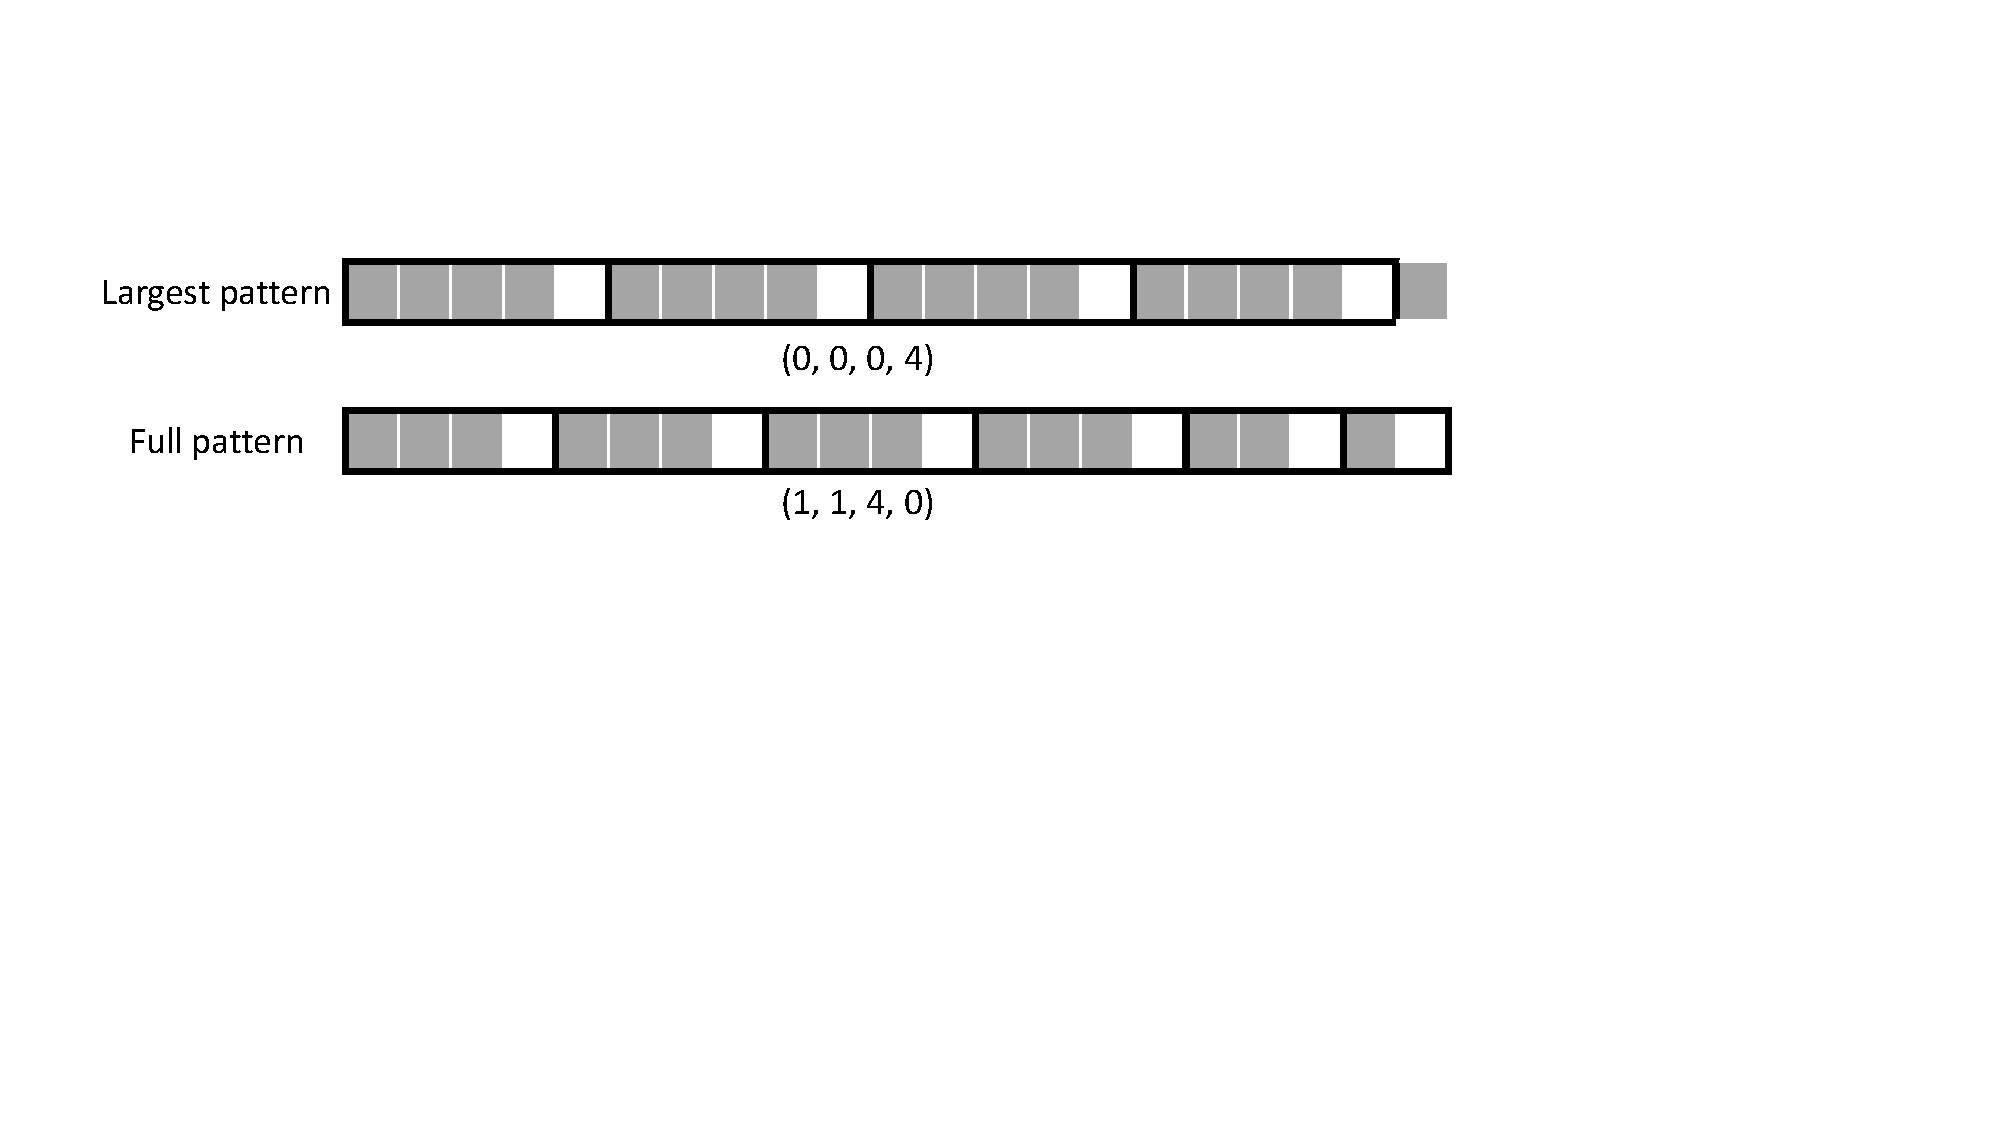
\includegraphics[width=0.8\textwidth]{./Figures/largest_full.pdf}
    \caption{Largest and Full Patterns}
\end{figure}

Pattern $(0, 0, 0, 4)$ is a largest pattern as its size is 16. However, it does not satisfy the requirement of fully utilizing all available seats since $4 \times 5 \neq 21$. Pattern $(1, 1, 4, 0)$ is a full pattern as it utilizes all available seats. However, its size is 15, indicating that it is not a largest pattern.
\end{example}

When the constraints \eqref{deter_upper} are tight while most constraints \eqref{capa_con} remain loose, indicating the availability of many seats, our goal is to derive a seat plan that maximizes seat utilization. This naturally leads to a related problem: given a feasible seat plan, we seek to obtain a seat plan that satisfies the original requirements of the feasible seat plan while utilizing as many seats as possible. Interestingly, the optimal seat plan consists of either full or largest patterns.


Let the feasible seat plan be $\bm{H}$ and the desired seat plan be $\bm{H}^{\prime}$. To satisfy requirements of planned group types in $\bm{H}$, the total quantity of groups from type $i$ to type $M$ in $\bm{H}^{\prime}$ must be at least equal to the total quantity from group type $i$ to group type $M$ in $\bm{H}$. Mathematically, we aim to find a feasible seat plan $\bm{H}^{\prime}$ such that $\sum_{k=i}^{M} \sum_{j=1}^{N} H_{kj} \leq \sum_{k=i}^{M} \sum_{j=1}^{N} H^{\prime}_{kj}, \forall i \in \mathcal{M}$. We say $\bm{H} \subseteq \bm{H}^{\prime}$ if this condition is satisfied.

To utilize all seats in the seat plan, the objective is to maximize the number of individuals that can be accommodated. Thus, we have the following formulation:

\begin{equation}\label{improve_seat}
  \begin{aligned}
  \max \quad & \sum_{i=1}^{M} \sum_{j=1}^{N} (n_i-\delta)  x_{ij} \\
  s.t. \quad & \sum_{k=i}^{M} \sum_{j=1}^{N}  x_{kj} \geq  \sum_{k=i}^{M} \sum_{j=1}^{N} H_{kj}, i \in \mathcal{M} \\
  & \sum_{i=1}^{M} n_{i} x_{ij} \leq L_{j}, j \in \mathcal{N} \\
  & x_{ij} \in \mathbb{N}, i \in \mathcal{M}, j \in \mathcal{N}
  \end{aligned}
\end{equation}

\begin{prop}\label{prop_construction}
Given a feasible seat plan $\bm{H}$, the optimal solution to problem \eqref{improve_seat} corresponds to a seat plan $\bm{H}^{\prime}$ such that $\bm{H} \subseteq \bm{H}^{\prime}$ and $\bm{H}^{\prime}$ is composed of either full or largest patterns.
\end{prop}


This approach guarantees the seat allocation with full or largest patterns while still accommodating the original groups' requirements. Furthermore, the improved seat plan can be used for the seat assignment when the group arrives sequentially.

